\section{Thursday, January 18th}
\subsection{Basic Definitions and Concepts}

Let \( \Omega = \{\text{set of all positive outcomes}\} \), \( w_j \in \Omega \) where \( w_j \) is a randomly chosen outcome.

Let \( |\Omega| = \) number of possible outcomes.

Let \( X(w_j) = x_j \), \( X: \Omega \rightarrow \mathcal{X} \) (our representation).

Let \( \Pr(w=w_j)=\Pr(X=x)=p_j \).

\begin{defn}{Intrinsic Functional}
An intrinsic functional is defined as \( U[X] = U(p) \), where \( U: \Delta_{|\Omega|} \rightarrow \mathbb{R} \)

Where \( \Delta_n \) is the simplex which is \( \{p \in \mathbb{R}^n , p_i \geq 0 \forall i \text{ and } \sum_{I=1}^n p_i = 1\} \) which geometrically looks like this image:
\begin{figure}[H]
    \centering
    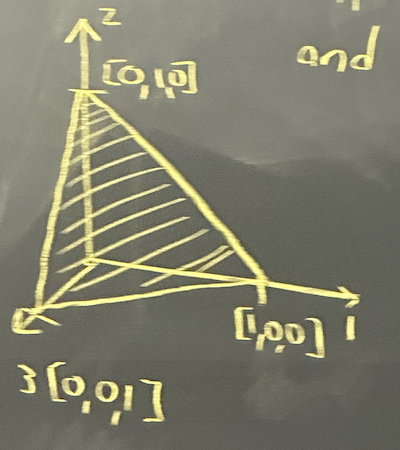
\includegraphics[scale=0.6]{lectures/wk1/img/simplex.png}
    \caption{Here we see a 3D-Simplex: a tetrahedron}
    \label{fig:simplex}
\end{figure}
\end{defn}

\subsection{Shannon Axioms}

\begin{defn}{Shannon Axioms}
Shannon axioms for a functional \( U: \Delta_n \rightarrow \mathbb{R} \), intrinsic:
\begin{itemize}
    \item Regularity/smoothness: \( U(p) \) is continuous in \( p \).
    \begin{itemize}
        \item Allows us to take limits: \( \lim_{x} f(x) = f(\lim_{x} x) \).
    \end{itemize}
    \item If \( p = [\frac{1}{n}, \ldots, \frac{1}{n}] \) ~ Uniform[\( n \)], \( |\Omega|=n \), then \( U(p) \) is non-increasing in \( n \).
    \item Uncertainty in \( X \) = Uncertainty in \( Y \) + Expected Uncertainty in \( X \) given \( Y \), for any choice \( \{S_1, S_2, \ldots\} \).
\end{itemize}
\end{defn}

\subsection{Khinchin Axioms}

\begin{defn}{Khinchin Axioms}
Khinchin axioms for a functional \( U: \Delta_n \rightarrow \mathbb{R} \), intrinsic:
\begin{itemize}
    \item \( U \) is intrinsic.
    \item For a given \( |\Omega| \), \( U(p) \) is maximized when \( p = [\frac{1}{\Omega}, \ldots, \frac{1}{\Omega}] \) aka uniform.
    \item Adding impossible outcomes (\( p_j = 0 \)) shouldn’t change your measure of uncertainty \( U(p) \).
    \item Chain Rule: \( U[X, Y] = U[Y] + \mathbb{E}_Y(U[X|Y]) \)
    \begin{itemize}
        \item Sometimes \( \mathbb{E}_Y(U[X|Y]) \) is written (mistakenly) as \( U[X|Y] \).
    \end{itemize}
\end{itemize}
\end{defn}

\subsection{Berkeley’s List of Axioms}

\begin{defn}{Berkeley’s Axioms}
Berkeley’s list of axioms:
\begin{itemize}
    \item \( U(p)=0 \) if \( p = [0, 0, \ldots, 0, 1, 0, \ldots, 0] \)
\end{itemize}
\end{defn}

\subsection{Composition}

Composition: If we partition \( \Omega \) into mutually exclusive and collectively exhaustive subsets \( S_1, \ldots, S_\psi \). 
Then let \( X \) represent the outcome in some subset.
Let \( Y \) be an indicator for the set containing \( X \): \( Y=j \) if \( X \in S_j \)
This is backwards from last class: here we will observe \( Y \) and estimate \( X \) in 2 stages:
\begin{enumerate}
    \item Observe \( Y \), we find that \( X \) is contained in some say \( S_1 \), which tells us that we are contained in a certain subset — but there’s still some uncertainty. So now we:
    \item Observe \( X \) given \( Y=y \).
\end{enumerate}
We want \( U[X] = U[Y] + \mathbb{E}_y(U[X | Y=y]) \).

\subsection{Shannon's Entropy Theorem}
\begin{defn}{Shannon's Entropy Theorem}
Given either Shannon’s or Khinchin’s axioms then:
\[ U[X]=U(p)=H[X]=H(p)=\text{``Shannon’s Entropy’’} \]
\[ = -\sum_{\text{all } x \in \mathcal{X}} \Pr(X=x) \log_a(\Pr(X=x)) \]
\[ = -\sum_{j=1}^{|\Omega|} p_j \log_a(p_j) \]
\[ = \mathbb{E}_X[\log_a(1/\Pr(X=x))] \]
Where:
\begin{itemize}
    \item By convention \( p=0 \implies p\log(p)=0 \) which is known as continuity and is proved by L’Hôpital’s as \( p \rightarrow 0^+ \) addressing Khinchin Axiom 3: \( H[p]=H[[p, 0, 0, 0]] \) as impossible events have 0 uncertainty.
    \item \( a \) is an arbitrary base which is a choice of unit to measure units (it is not uniquely specified by the axioms).
    \begin{itemize}
        \item \( \log_2 \implies \) “bits”
        \item \( \log_3 \implies \) “ternary function”
        \item \( \ln \implies \) “nats”
        \item All of these are off by a scaling factor, as shown below,
    \end{itemize}
\end{itemize}
\end{defn}

\subsection{Logarithmic Change of Base for Entropy}
$$
\log _b a=\frac{\log _d a}{\log _d b}
\implies 
H_b(p) = \log_b(a) H_a(p).
$$
